\section{IEEE 802.15.4e}\label{sec:etat_art-802.15.4}
\renewcommand{\rightmark}{IEEE 802.15.4e}
    802.15.4 est un protocole définis par IEEE en 2003. Il est destiné aux communications à débit faibles réalsisées par des dispositifs ayant une alimentation en énergie limitée.
    Ce protocole qui est un standart pour les réseaux PANs (Personak Area Networks) couvre la couche physique et MAC du modèle OSI.


\subsection{Types de noeuds}\label{subsec:etat_art-802.15.4.nodes}
  La norme 802.15.4 défini deux types de noeuds:
  \begin{itemize}
    \item Les noeuds \textbf{FFD} (Full Function Device) peuvent être des corrdinateurs de PAN, de simple
          coordinateurs ou de simple noeuds.
    \item Les noeuds \textbf{RFD} (Reduced Function Device) utilisent une implémentation réduite du protocole
    et peuvent seulement opérer comme des simples noeuds.  
  \end{itemize}

  Ces noeuds peuvent former des réseaux suivantes plusieurs topologies
  comme la topologie en étoile pour laquelle plusieurs RFD sont connectés à un FFD qui
  joue le rôle de coordinateur ou encore la topologie peer-to-peer pour laquelle les FFD sont connectés les uns aux autres.


\subsection{Beacon Enabled mode}\label{subsec:etat_art-802.15.4.be}
  Dans ce mode d'accès, le réseau est synchronisé par des messages de contrôles (beacons)
  et une structure appelée Superframe (Fig. \ref{fig:etat_art-802.15.4.superframe}).
  
  La superframe est divisée en deux périodes: la période active et la période inactive.

  La période active est elle-même divisée en deux périodes:
  \textit{contention acces period (CAP)} et \textit{contention free period (CFP)}.

  \begin{figure}[H]
    \centering
    \makebox[\textwidth]
    {
      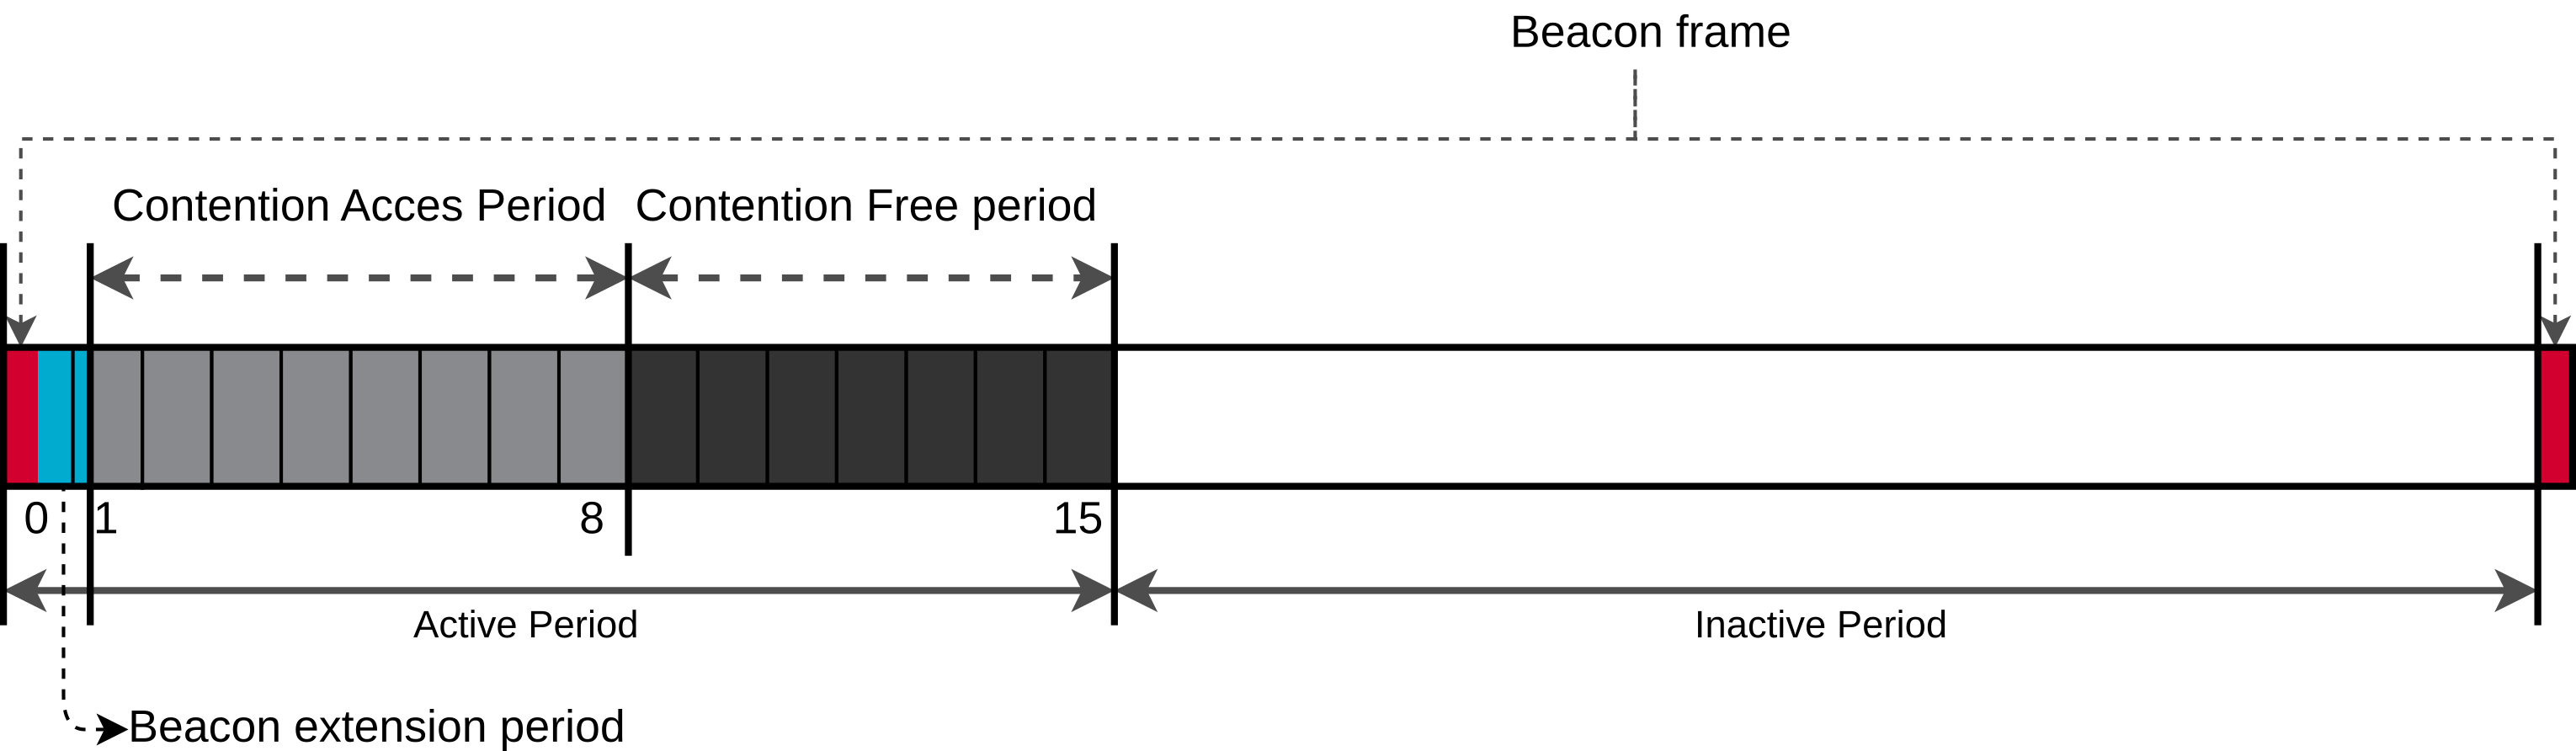
\includegraphics[scale=0.8]{images/superframe.png}
    }
    \caption{802.15.4 structure de la Superframe.}
    \label{fig:etat_art-802.15.4.superframe}
  \end{figure}

\subsubsection*{Accès au canal durant la contention acces period (CAP)}
  Durant cette période, l'accès au canal se fait par l'algotihme slotted CSMA-CA
  (Carrier Sense Multiple Access with Collision Avoidance). La figure~\ref{fig:etat_art-slotted_csmaca}
  illustre son fonctionnement.

  Les time slots de la CAP sont divisés en plus petits time slots appelés \textbf{backoff periods}.
  Un noeud du réseau maintient les variables suivantes:
  \begin{itemize}
    \item $NB$ compte le nombre de backoff. Initialisée à 0
    \item $CW$ indique la taille de la fenêtre de congestion. Initialisée à 2
    \item $BE$ est l'exposant du backoff. Initialisée à macMinBE
  \end{itemize}

  Les variables macMinBE, macMaxBe et MCB (macCSMABackoffs) sont des constantes du protocole.
  Lorsque des paquets doivent être transmis, les variables sont d'abord initialisées.
  Ensuite, le noeud attend le prochain backoff et choisis aléatoirement un nombre entier
  $r r \in [0, 2^{BE}-1]$. Après avoir avoir attendu r backoff periods, le noeud vérifie
  si le canal est occupé en réalisant un CCA (Clear Channel Assessment).
  Si c'est le cas, $CW$ va être décrémenté et un nouveau CCA va être réalisé.
  Les paquets ne pourront être transmis qu'après trois CCA consécutifs indiquant un canal libre (i.e. $CW = 0$).
  Si le canal est occupé, $NB$ et $BE$ sont incrémentés et $CW$ est réinitialisé à 2.
  Enfin, si $NB$ n'exède pas \textit{macCSMABackoffs}, le noeud va reprendre à l'étape où un
  $r$ est choisis aléatoirement. Sinon, la communication ne sera pas établie et les paquets
  ne seront pas transférés.


\begin{figure}[H]
  \centering
\begin{tikzpicture}[node distance=1.7cm, scale=0.85, every node/.style={scale=0.85}]

  \node (start) [process] {\begin{tabular}{c} $NB = 0$; $CW = 2$ \\ BE = macMinBE \end{tabular}};
  \node (in1) [process, below of=start] {\begin{tabular}{c} wait until next backoff\\ period boundary\end{tabular}};
  \node (pro1) [process, below of=in1] {\begin{tabular}{c} Skip $r \in [0, 2^{BE}-1]$ \\ backoff periods \end{tabular}};
  \node (pro2) [process, below of=pro1] {Perform CCA};
  \node (dec1) [decision, below of=pro2, yshift=-0.8cm] {Channel idle?};

  \node (pro2a) [process, below of=dec1, yshift=-1cm] {\begin{tabular}{c} $NB = NB+1;CW = 2$ \\ $BE = min(BE+1, macMaxBE)$ \end{tabular}};
  \node (pro2b) [process, right of=pro2a, xshift=4cm] {$CW = CW-1$};
  \node (dec2) [decision, below of=pro2a, yshift=-1cm] {NB > MCB ?};
  \node (dec3) [decision, below of=pro2b, yshift=-1cm] {CW = 0\ ?};
  \node (fail) [endfail, below of=dec2, yshift=-1cm] {Failure};
  \node (success) [endsuccess, below of=dec3, yshift=-1cm] {Success};
  
  \draw [arrow] (start) -- (in1);
  \draw [arrow] (in1) -- (pro1);
  \draw [arrow] (pro1) -- (pro2);
  \draw [arrow] (pro2) -- (dec1);
  \draw [arrow] (dec1) -| node[anchor=south] {Yes} (pro2b);
  \draw [arrow] (dec1) -- node[anchor=east] {No} (pro2a);
  \draw [arrow] (pro2a) -- (dec2);
  \draw [arrow] (pro2b) -- (dec3);
  \draw [arrow] (dec2) -- node[anchor=east] {Yes} (fail);
  \draw [arrow] (dec2) -- node[anchor=south] {No} ++(-4,0) |- (pro1);
  \draw [arrow] (dec3) -- node[anchor=south] {No} ++(3,0) |- (pro2);
  \draw [arrow] (dec3) -- node[anchor=east] {Yes} (success);
  \end{tikzpicture}
  \caption{Schéma de l'algorithme slotted CSMA-CA.}
  \label{fig:etat_art-slotted_csmaca}
\end{figure}


\subsubsection{Accès au canal durant la contention free period (CFP)}
Le mécanisme utilisé durant cette phase d'accès est TDMA (Time Division Multiple Access).
Comme illustré sur la figure~\ref{fig:etat_art-802.15.4.superframe}, cette période est divisée
en 7 slots qui sont attribués par le coordinateur aux noeuds ayant émis une GTS (Guaranteed
time slots) durant la période de CAP.
Cette requête spécifie le nombre de slots consécutifs désirés ainsi que le type de slot demandé:
slot de transmission ou de réception.
Après réception de cette requête, le coordinateur va répondre en deux temps. D'abord, un ack pour
confirmer la réception de la requête et ensuite un beacon appelé GTS descriptor lorsque les ressources
demandées sont disponibles.

\subsection{Non-Beacon Enabled mode}\label{subsec:etat_art-802.15.4.nbe}
Ce mode d'accès n'utilise pas de beacons. Il n' a donc aucune synchronisation.
L'accès au canal se fait alors par l'algorithme Unslotted CSMA-CA illustré par la
figure~\ref{fig:etat_art-unslotted_csmaca}. On remarque que cet algorithme est similaire
à soltted CSMA-CA à l'expection que le CCA est réalisé qu'une seule fois et que l'algortihme
n'attend plus un time slot du CAP avant d'attendre un nombre de backoff aléatoire.

\begin{figure}[H]
  \centering
\begin{tikzpicture}[node distance=1.7cm, scale=0.8, every node/.style={scale=0.8}]

  \node (start) [process] {\begin{tabular}{c} $CW = 2$ \\ BE = macMinBE \end{tabular}};
  \node (pro1) [process, below of=in1] {\begin{tabular}{c} Skip $r \in [0, 2^{BE}-1]$ \\ backoff periods \end{tabular}};
  \node (pro2) [process, below of=pro1] {Perform CCA};
  \node (dec1) [decision, below of=pro2, yshift=-0.8cm] {Channel idle?};

  \node (pro2a) [process, below of=dec1, yshift=-1cm] {\begin{tabular}{c} $NB = NB+1$ \\ $BE = min(BE+1, macMaxBE)$ \end{tabular}};
  \node (dec2) [decision, below of=pro2a, yshift=-1cm] {NB > MCB ?};
  \node (fail) [endfail, below of=dec2, yshift=-1cm] {Failure};
  \node (success) [endsuccess, right of=fail, xshift= 4cm] {Success};
  
  \draw [arrow] (start) -- (pro1);
  \draw [arrow] (pro1) -- (pro2);
  \draw [arrow] (pro2) -- (dec1);
  \draw [arrow] (dec1) -- node[anchor=east] {No} (pro2a);
  \draw [arrow] (pro2a) -- (dec2);
  \draw [arrow] (dec2) -- node[anchor=east] {Yes} (fail);
  \draw [arrow] (dec2) -- node[anchor=south] {No} ++(-4,0) |- (pro1);
  \draw [arrow] (dec1) -| node[anchor=south] {Yes} (success);
  \end{tikzpicture}
  \caption{Schéma de l'algorithme unslotted CSMA-CA.}
  \label{fig:etat_art-unslotted_csmaca}
\end{figure}

\subsection{80.15.4e}\label{subsec:etat_art-802.15.4.limitations}
802.15.4 a un certains nombres de limitations:
\begin{itemize}
  \item Aucune garantie sur le délai maximal pour qu'un paquet puisse atteindre sa destination
    ne peut être fourni avec l'alorithme CSMA-CA.
  \item La fiabilité des communications est limitée par l'utilisation de l'algorithme slotted CSMA-CA
    qui offre un taux de transmission faible.
  \item Aucune protection contre les interférences due à l'utilisation d'un seul canal et à l'absence
    de mécanismes de sauts de fréquence (frequency hopping)
\end{itemize}
Ces limitations ont menées à la création de 802.14.4.e qui redifinis les protocoles MAC du standard.

Ainsi, 5 modes de fonctionnement de la couche MAC sont définis:
\begin{enumerate}
  \item \textbf{Time Slotted Channel Hopping (TSCH)}\\
    %Cible les applications tel que l'automatisation de processus. Permet des communications %multi-sauts et multi-canaux.
  \item \textbf{Deterministic and Synchronous Multi-channel Extension (DSME)}\\
    %Réalisé pour des applications industirelles et commercialesayant des contraintes de délai et
    %fiabilité. Permet des communications multi-sauts ainsi que la création de réseaux MESH.
  \item \textbf{Low Latency Deterministic Network (LLDN)}\\
    %Conçu pour les applications nécessitant une latence faible et les réseaux n'utilisant qu'un seul
    %canl pour des chemins d'un saut maximum.
  \item \textbf{Asynchronous multi-channel adaptation (AMCA)}\\
    %Cible les applications où de grands déploiments sont nécessaire comme le monitoring %d'infrastructures.
  \item \textbf{Radio Frequency Identification Blink (BLINK)}\\
    %Conçu pour i'identification de personnes ou d'objets. Il permet aux noeuds de communiquer leur
    %ID aux autres noeuds sans avoir été préalablement associés.
\end{enumerate}

\subsection{TSCH (Time Slotted Channel Hopping)}\label{subsec:etat_art-802.15.4.tsch}

Ce mode de fonctionnement de la couche MAC, comme son nom l'indique, supporte à la fois les sauts en fréquence et des communications divisées en temps.\\

\textbf{Slotframe}\\
Dans ce mode, le concept de superframe de 802.15.4 est remplacé par le concept de slotframe.
Une slotframe est un intervalle de temps qui divisé en timeslots. Chaque timeslot permet à un noeud d'envoyer une trame et d'éventuellement recevoir son acquitement (ack).
Chaque timeslot possède un identifiant appellé \textit{Absolute Slot Number} (ASN) ...
et un identifiant au sein de la slotframe appelé \textit{Time Slot Number} (TSN).

La figure \ref{todo} illustre une slotframe composée de trois timeslots.
Dans cet exemple, on considère 3 noeuds: N, T et U. Chaque timeslot permet une communication.
Par exemple le timeslot ayant comme TSN 0, permet à N de transmettre vers T.

\begin{figure}[H]
  \centering
  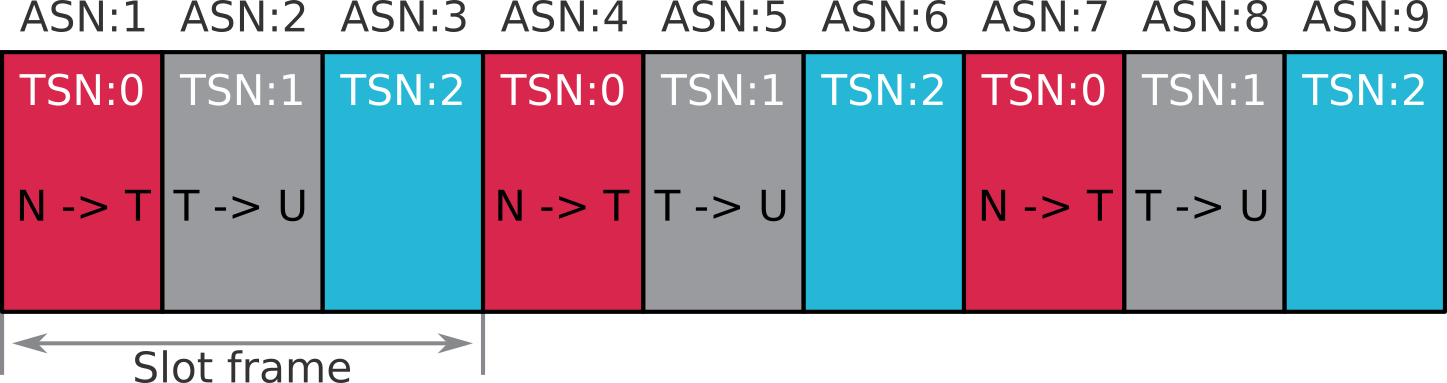
\includegraphics[scale=0.7]{images/sloframe.png}
  \caption{Slotframe}
  \label{todo}
\end{figure}

\textbf{Channel Hopping}\\

TSCH peut utiliser 15 canaux différents numérotés de 0 à 15.
